\chapter{Road Writer}

\begin{figure}[H]
    \centering
    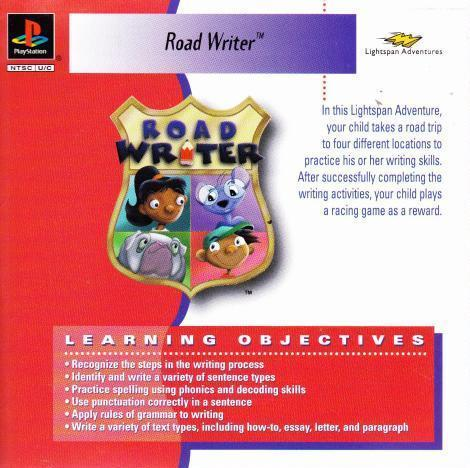
\includegraphics[width=0.5\textwidth]{"./Games/RoadWriter/Images/RoadWriterCDCover.jpg"}
    \caption{Official RoadWriter PlayStation 1 CD Cover}
\end{figure}

Road Writer for the PlayStation 1 is one of the only games within the Lightspan Adventures series that exists on its own as its own game, as opposed to as part of a series.
The game is designed to help children to practice and improve their writing skills.

In addition, it appear to be one of the few games which allow you to save you progress, in order to continue where you left off.

The game consists of two difficultly settings: Export and Pro.
Depending on the difficulty the player selects, they will have a variety of different locations to explore within the game.

The Expert difficulty setting has the following locations:

\begin{itemize}
    \item Mount Hans
    \item LaMancha Canyon
    \item Dodgson Creek
    \item New Bronzeville
\end{itemize}

The Pro difficulty setting has the following locations:

\begin{itemize}
    \item Canterbury Canyon
    \item Greene Woods
    \item Hamlet Springs
    \item Hughes City
\end{itemize}

For each location, no matter the difficult, the player is able to select from a variety of writing minigames:

\begin{itemize}
    \item Writing Assignment
    \item Prewriting (contains two difficulties: level 1 and level 2)
    \item Revising (contains two difficulties: level 1 and level 2)
    \item Proofreading (locked until the player has completed the other three minigames)
\end{itemize}

\section{Transcriptions}

\subsection{Home Screen - Chaucer}

A globe-trotter, Chaucer's travelled through every continent.
Author of 'It's a Dog's Life', Chaucer is current editor of the very popular 'Dog Year' magazine.

\subsection{Home Screen - Ralph}

An experience political journalist, Ralph has walked with every US presidents dog in office.
A careful and intelligent listener, he has scooped many an unwitting hound by getting the story first, straight from the first dog's kennel.

\subsection{Home Screen - Gwyn}

A poet, short story writer and reporter for the high school paper, Gwyn is alway ready to pick up a new story or a quick game of hoops.
A crusader for human rights, Gwynn is the go-to person, and take the ball hard to the hoop.

\subsection{Home Screen - Miguel}

Whether it's investigating a political coverup, or sleuthing business fraud, Miguel is the champion of integrity.
His goal is to have a Pulitzer Prize by 21, so he races from class to city hall to his privately published newsletter, which he calls 'Don Quixote'.
Count on him to get the news out and let the public decide.

\subsection{Road Writer Song}

Gotta write a story, got something to say,

You're on the right road, gotta say it our way,

Our story unfolds, we're on the right road,

Nobody can see the world exactly like we do,

Nobody can write about like me and you,

Like you,

Gotta think it up, and write it down,

Gotta share it with a friend,

Changing it, rearranging it,

Fine tune it to the end,

Let the story unfold, just get on the right road,

Get going now, get on the move,

Start writing, do it today,

Every road's original, gotta say it all our way,

Gotta see the world exactly like we do,

We're on the right road, the right road

\subsection{Writing Assignment - Introduction}

MIGUEL:
Don't panic, it's essay time.
Do it step by step.
First, decide on the main idea.

GWYN:
Next, jot down an outline of the key points that support the main idea.

MIGUEL:
Right Gwyn.
To sum it up, every essay needs an introduction to the main idea, two or three paragraphs that support the main idea, and a conclusion.
So let's get rolling.

\subsection{Writing Assignment - Conclusion}

MIGUEL:
Excellent essay!
It's a real gem.

GWYN:
A goldmine of creativity!

MIGUEL:
Let's put the pedal to the medal and write on!

\section{Credits}

Concept by: Margy Hillman,
Story written by: Margy Hillman, Jon Silver,
Vice President, Product Design: Margy Hillmaan,
Director, Interactive Product Design: Lourdes Bouras,
Senior Program Manager: Kevin Clark,
Lead Content Designer: Alma Torres,
Content Designers: Amy Nicholson, Ann Rybowiak,
Senior Porgram Manager, Curriculum: Sherri Furqueron,
Curriculum Specialists: Margie Glickman Jones, Christina Roll,
Content Writers: Melanie Brannan, Sarah Curry, Kristen Enyedi, Paige Gushaw, Christina Roll,
Editor: Julia Hagen,
Curriculum Consultants: James Flood, Ph.D., Dianne Lapp, Ed.D.,
Interactive Game Coordinators: Laurie Miles, Kristin Rix,
Senior Manager, Product Implementation Materials: Judy Carr,
Curriculum Support: Aimée Bachmann, Shelly Crickett,
Writer: John Dorsey,
Desktop Publisher: Dave Mauch,
Student Contributors: Brittany Acompora, Leah Bolosan, Beatriz Bouras, Eric Bradford, Kyle Brewer, Chelsea Clay, Aaron DeLeon Guerrero, Kate Franz, Brittney Gordon, Brian Hill, Danny Kuszmaul, Richard Mayer, Alex Merrill, Mitchell Scherimer,
Mason Elementary: Ms. Beisch's class, Ms. Borkenhagen's class, Ms. Talner's class, Ms. Trigg's class,
Meridian Elementary: Ms. Bassett's class, Ms. Calvao's class, Ms. Kinard's class, Ms. Kleis' class, Ms. Taggart's class,
Oak Park Elementary: Ms. Goss' class, Ms. Le Tourneau's class,
Rios Elementary: Ms. Larson's class, Ms. Maloney's class, Ms. Perry's class,
Rock Spring Elementary: Ms. Grossman's class, Ms. Wright's class,
Valencia Park Elementary: Ms. Davies' class, Ms. Hedgren's class,
New Bridge Elementary: Ms. Mayo's class,
Vice President, Studio Production: Margy Hillman,
Executive Producer: David Hamby,
Animation Producer: Al Lowenheim,
Interactive Producer: David Adams,
Associate Producer: Jon Silver,
Production Manager: Janet Dahle,
Director, Media Production Technologies: D. Scott Murdoch,
Assistant Art Director: Ken Anderson,
Unit Manager, Preproduction and 2-D: Jan Hastings,
Assistant Directors: Luther McLaurin, Steve Merghart,
Pose Artists: Luther McLaurin, Jeff Merghart,
Lead Animators: Burt Julio, Rosemary Rodgers, Virgil Sanico, Stania Vagner,
Animators: Gene Stout,
Layout Artist: Gene Stout,
Unit Manager, Interactive: Eydie Gilley,
Prototype Artist: Bryon Rodarmel,
Lead Game Artists: Callie Mack, Long Phan, Suzy Sadak, Judy Temple,
Background Artists: Edgardo Magsino,
Graphic Artists: Nora Read, Christina Wilson, Amy Zeller,
Manager, 3-D: Eric Fuss,
Digital Ink and Paint: Katherine Laxa, Melanie Strauss,
Unit Manager, Post Production and 3-D: Colleen McPhillips,
Audio Producer: Rick Bowman,
Audio Engineer: Brad Aldredge,
Voice Talent: Beatriz Bouras, Connor Bringas, Corey Bringas, Deem Bristow, Steve Brodie, Charles Cox, Jr., Suzanne Dean, Ryan Drummond, Jocelyn Raquel Freitas, Katie Heinemann, Deanna Hurst, Joel Ressel, Richie Ressel, Kendall Sczempka, Erik Thompson, Sarah Vincelett,
Music: Ken Ashby, Mike Peed,
Production Control Technician: David Martin,
Technical Editor: Lori Silfen,
Data Management Assistant: Sjoukie Cooper-Holt,
Asset Management Supervisor: Monica Chernus,
Asset Management Assistant: Katharine Laxa,
Executive Administrator: Rae Farley,
Vice President, Product Development: Sergio Garcia,
Director, Software Technology: William Volk,
Project Manager: Robert Warren,
Lead Software Engineer: Glenn Kalani,
Software Engineers: Tom Birchall, Ned Wallace,
Graphic Artist: Joy Schmalfeldt,
Production Assistant: Tonette Salter,
Programming Intern: Jeston Furqueron,
Quality Assurance Manager: Mark Myers,
Quality Assurance Supervisor: Fred Pecoroni,
Quality Assurance Analysts: James Cajala, Parish Goynes, Randy Jones, Jenna Payne, Janet Row, Geno Vici, Tony Vo,
Quality Assurance Testers: Kevin Garcia, David Hickson, Barbara King, Richard Kriegler, Bill O'Bannon, Ines Panchenko, Barry Rader, Kathy Taylor, Marlan Wilson